
\chapter{Addressing Serialization Errors by Discarding Sequential Position Information}
\label{chapter:chapter4}

\renewcommand{\leftmark}{\spacedlowsmallcaps{Addressing Serialization Errors by Discarding Sequential Position Information}}

\begin{chapabstract}
    {\em
    Chapter Abstract


    \vspace*{5mm}
    The work in this chapter has led to the submission of a paper currently under review:}
    \begin{itemize}
        \item \small \fullcite{}.
    \end{itemize}
\end{chapabstract}

\ifthenelse{\boolean{skipCh4}}{\endinput}{}


\newpage

\minitoc
\chapterwithfigures{\nameref*{chapter:chapter4}}
\chapterwithtables{\nameref*{chapter:chapter4}}

Textual content is organized in a specific order to convey meaning and context.Hence, reading order is crucial for models to perform well because it reflects the natural flow and structure of information in a document. When models are trained with a reading order that aligns with human understanding, they learn to capture the relationships between words, sentences, and paragraphs. 

Most pre-training methods for Document Understanding rely on serialized text, where either an \ac{OCR} system or a PDF parser is used to extract text. However, \textit{serialization errors}, \textit{i.e.}, inaccuracies or issues that arise during text extraction, may arise and lead to misinterpretations, distortions, or misalignments in the extracted text when compared to the original visual content. For instance, an \ac{OCR} system might misinterpret or introduce extraneous characters, while a PDF parser might misinterpret formatting elements or misorder words. Most of the time, the text extracted is re-arranged in a raster-scan order, aligning tokens from the top-left to the bottom-right corner. However, this linear organization does not always align with human reading patterns, particularly in documents with complex layouts such as multicolumn texts, tables, and forms. Serialization errors impact the accuracy of the extracted text and, therefore, the entire text processing pipeline. Without an accurate reading order, models may misinterpret the relationships between different parts of the text, resulting in suboptimal performance in downstream tasks. This poses a substantial challenge in various applications, notably Document Understanding, where document layouts can be complex. 

On the other hand, layout inherently encapsulates the correct reading order of documents by visually organizing content in a structured manner. A well-designed layout guides the reader's natural progression from one section to another, ensuring coherent and logical information flow. Therefore, understanding the layout provides essential cues for determining the correct reading order, as it aligns with the visual hierarchy and structure intended by document creators. 

Yet, existing pre-training methods for Document Understanding often neglect this aspect, opting to oversimply the integration of layout by adding it as an extra embedding in the input layer \citep{xu2020layoutlm} or as a bias term in the attention layer \citep{xu2020layoutlmv2}. ERNIE-Layout \citep{peng2022ernie} stands out as one of the few endeavors that consider errors introduced by OCR serialization. While the model learns the relationship between layout and reading order through a pre-training strategy involving reading order prediction, it continues to rely on sequential position embeddings derived from the reading order obtained via \ac{OCR}. However, \citet{haviv2022transformer} show that causal language models without any explicit positional encodings develop an implicit understanding of absolute positions, compensating for missing information. It is suggested that causal attention allows the model to estimate the number of predecessors each token can attend to, approximating its absolute position. Our objective is to show that this can be a general case (\textit{i.e.}, with bidirectional attention) when layout information is provided.

In this chapter, we focus on mitigating serialization errors by entirely discarding sequential position information. We introduce \textit{Layout2Pos}, a novel module designed to generate 1D position embeddings from the document layout by learning to reconstruct the relative order between tokens. Our endeavor is twofold: from a practical standpoint, we aim to enhance the robustness of models to reading order changes, crucial for real-world applications; from a theoretical perspective, we demonstrate that it is feasible to discard sequential position information without compromising overall performance. We incorporate this module into sequence-to-sequence models for visual information extraction tasks, eliminating the reliance on reading order during the entity extraction process.

% We attribute the improvement to the fact that, although the advanced serialization is not used for fine-tuning datasets, the model has the ability to understand the proper reading order of documents after pre-training.

% \section{Preliminary Experiments: OCR Errors}

% Preliminary experiments on ReadingBank

\section{Reconstructing Positional Information from 2D Positions}

\todo[inline]{Intro}

\subsection{Preliminary Experiments: OCR Serialization Errors}

To gauge the extent of \ac{OCR}-induced serialization errors, we conduct preliminary experiments comparing the reading order produced by Tesseract \citep{kay2007tesseract}, a widely-used \ac{OCR} system, against the annotated ground-truth reading order. The goal is to assess the alignment of the reading order produced via \ac{OCR} with the actual human reading patterns.

We use a subset of 100 documents from the ReadingBank \citep{wang2021layoutreader} dataset. ReadingBank is a benchmark dataset for reading order detection that includes high-quality reading order annotations extracted from Word documents. These annotations capture the correct sequence of words as visually presented in the documents. For our analysis, we categorize the document layouts into four types observed in the samples: \textit{plain} layout, \textit{lists}, \textit{multicolumn} layout, and \textit{tables}. We provide examples in Figure~\ref{fig:layout-examples}.

Tesseract is employed to extract and serialize text from the documents. The reading order produced by Tesseract is compared against the ground-truth for discrepancies. Specifically, we evaluate accuracy by comparing, for each word in the ground-truth sequence, the actual next word with the next word in the sequence generated by Tesseract. We compute the accuracy obtained for each specific layout type. Results are reported in Table~\ref{table:ocr-preliminary-experiments}. Our findings indicate that Tesseract faces increased difficulty in reconstructing the correct reading order as the document layout becomes more complex.\footnote{This difficulty in accurately predicting the next word is further attributed to the \ac{OCR}'s misinterpretation of certain words.} Additionally, we provide the ground-truth reading order and the reading order generated by Tesseract for a sample table (Figure~\ref{fig:reading-orders-table}) and a document with a multi-column layout  (Figure~\ref{fig:reading-orders-multicolumn}). In the case of the table, a comparison with the ground-truth reading order reveals that Tesseract lacks knowledge about cells, as it organizes text in a top-left to bottom-right manner. Regarding the document with two columns, Tesseract reads the text column by column, despite the document being horizontally divided into subgroups. This observation highlights Tesseract's limited understanding of the text's structure. 

These preliminary experiments provide the groundwork for investigating into novel approaches designed to alleviate serialization errors, ultimately enhancing the performance of document understanding models.

\begin{figure}[!htbp]
    \centering
    \small
      \begin{subfigure}[b]{0.24\textwidth}
        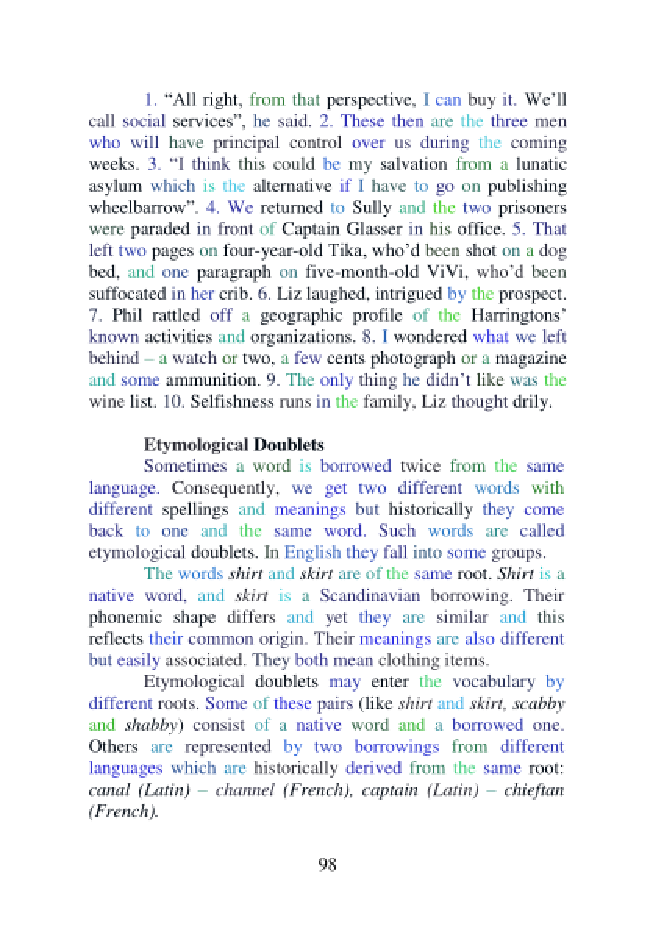
\includegraphics[width=\textwidth]{images/chapter4/plain.pdf}
        \caption{Plain}
      \end{subfigure}
      \begin{subfigure}[b]{0.24\textwidth}
        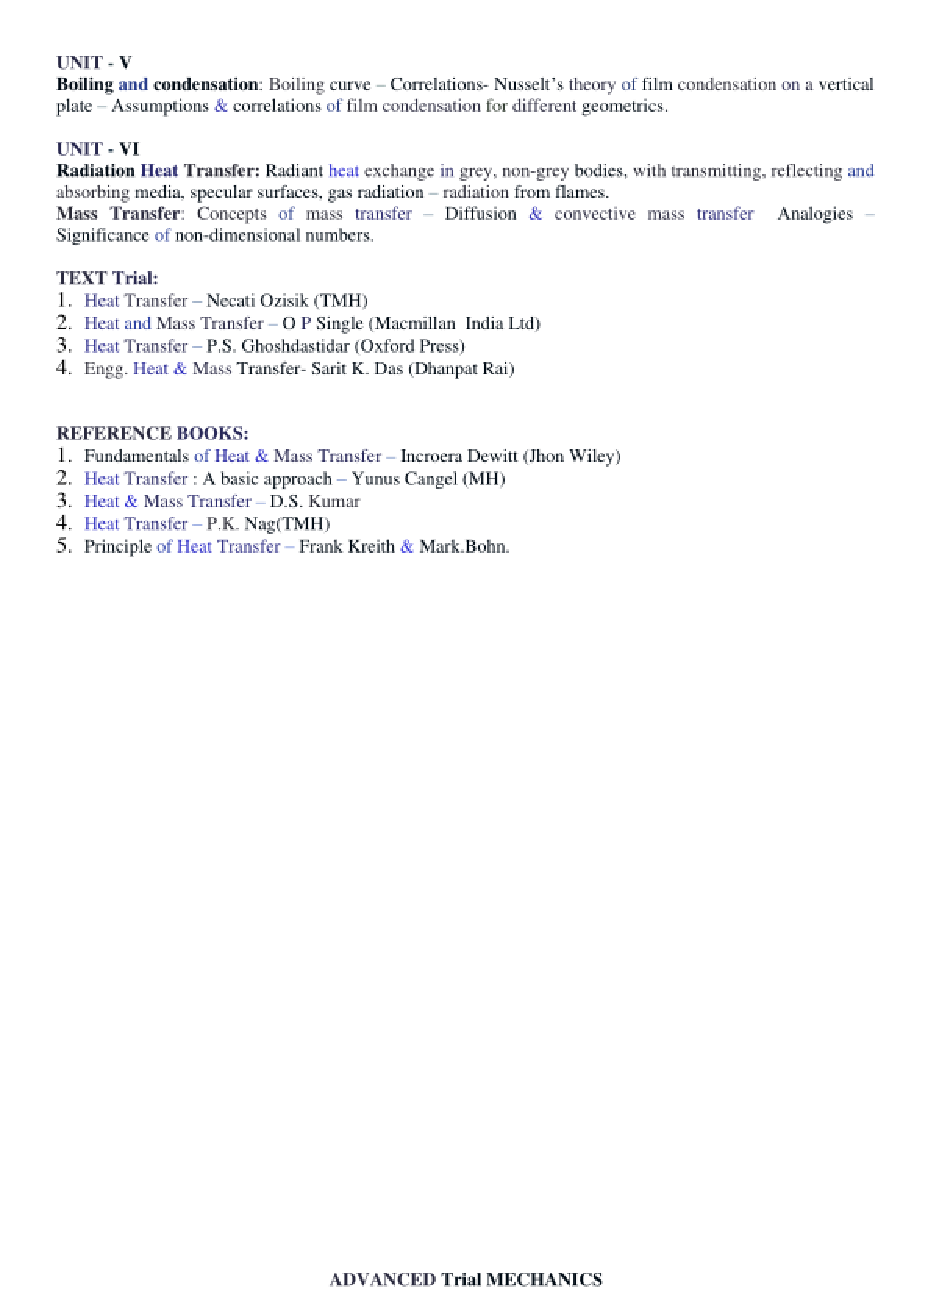
\includegraphics[width=\textwidth]{images/chapter4/list.pdf}
        \caption{List}
      \end{subfigure}
      \begin{subfigure}[b]{0.24\textwidth}
        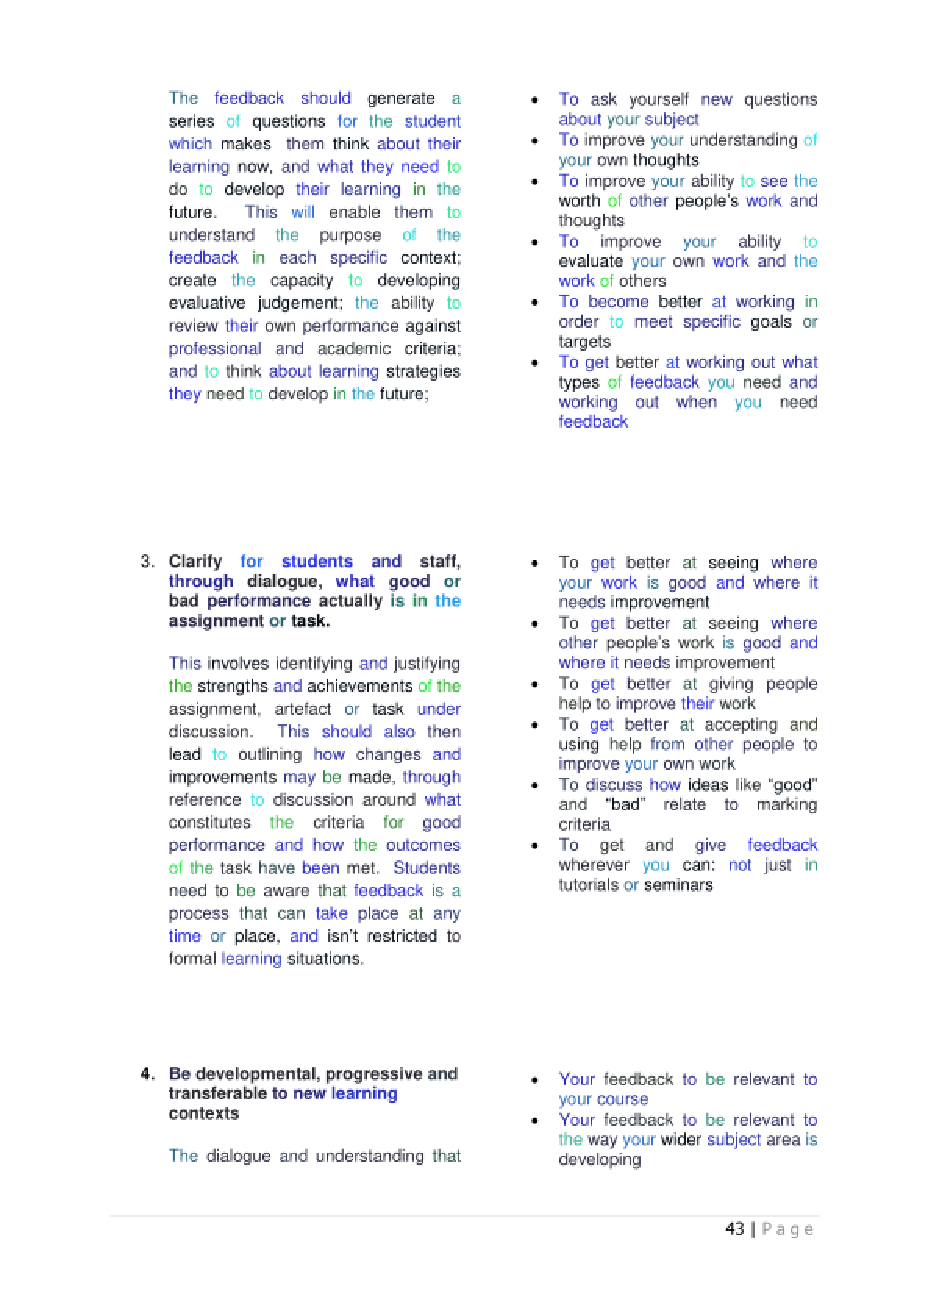
\includegraphics[width=\textwidth]{images/chapter4/multicolumn.pdf}
        \caption{Multicolumn}
      \end{subfigure}
      \begin{subfigure}[b]{0.24\textwidth}
        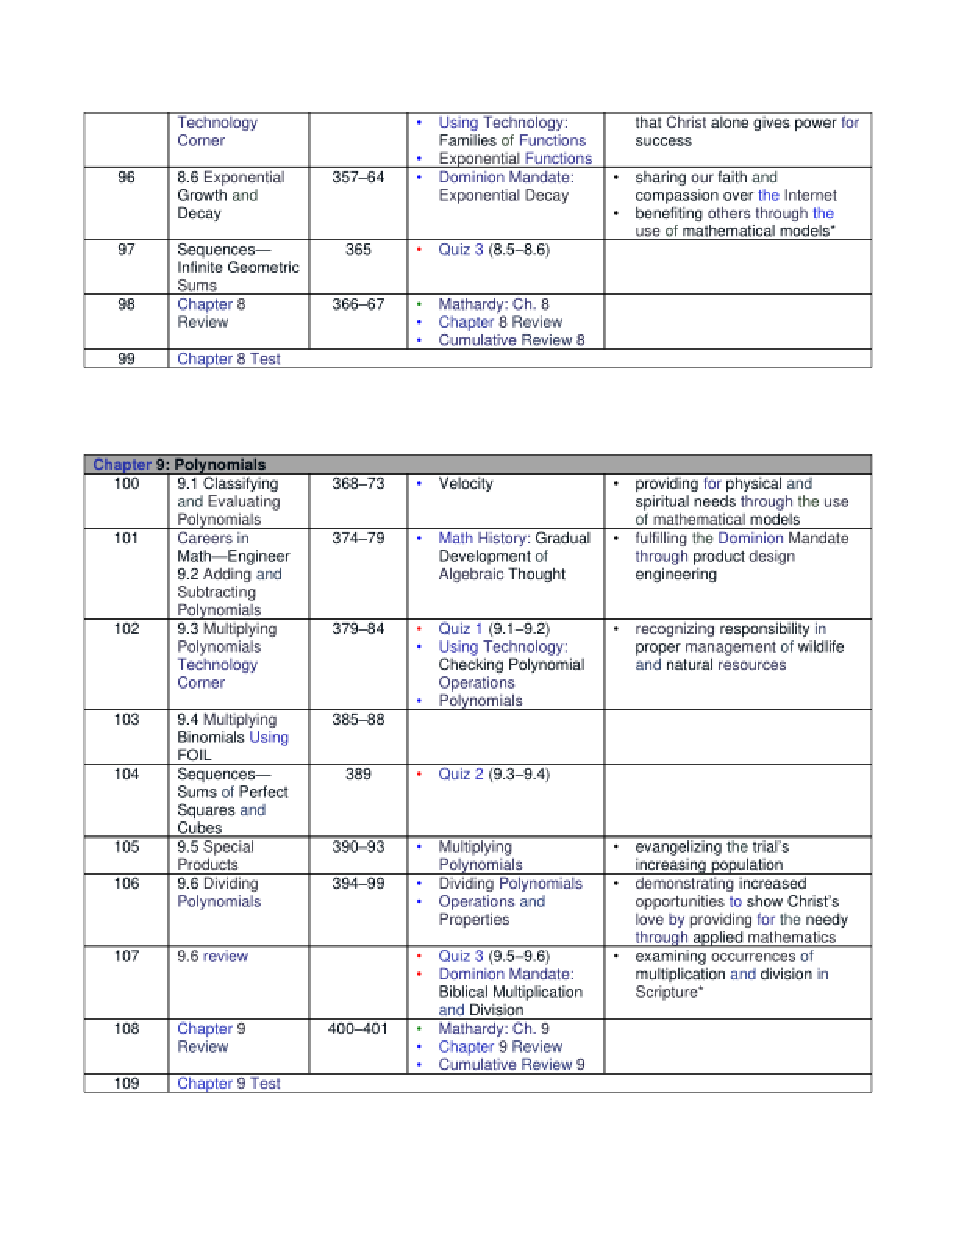
\includegraphics[width=\textwidth]{images/chapter4/tables.pdf}
        \caption{Table}
      \end{subfigure}
    \caption{Examples of documents for each layout category, arranged from the simplest to the most complex.}
    \label{fig:layout-examples}
\end{figure}

\begin{table}[!htbp]
  \centering
  \small
  \begin{adjustbox}{max width=\textwidth}
  \begin{threeparttable}
  \begin{tabular}{lcccccccc}
      \toprule
          % \multicolumn{4}{c}{\textbf{Layout Type}} & \\
          \textbf{Plain} & \textbf{Lists} & \textbf{Multicolumn} & \textbf{Tables}\\
      \midrule
      78.71\% & 72.75\% & 61.43\% & 36.97\%\\
  \bottomrule
  \end{tabular}
  \end{threeparttable}
  \end{adjustbox}
  \caption{Accuracy obtained for each document layout type.}
  \label{table:ocr-preliminary-experiments}
  \end{table}

\begin{figure}[!htbp]
    \centering
    \small
      \begin{subfigure}[b]{\textwidth}
        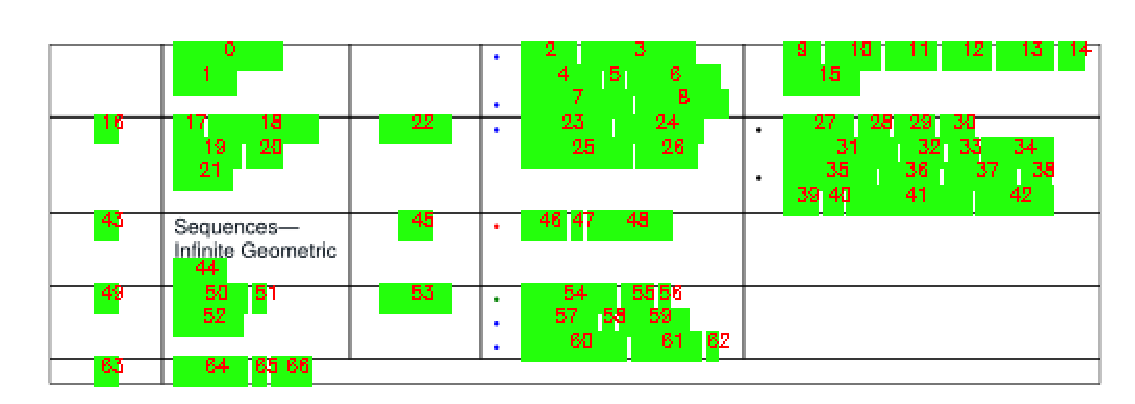
\includegraphics[width=\textwidth]{images/chapter4/gold_tables.pdf}
        \caption{Ground-truth reading order}
      \end{subfigure}
      \begin{subfigure}[b]{\textwidth}
        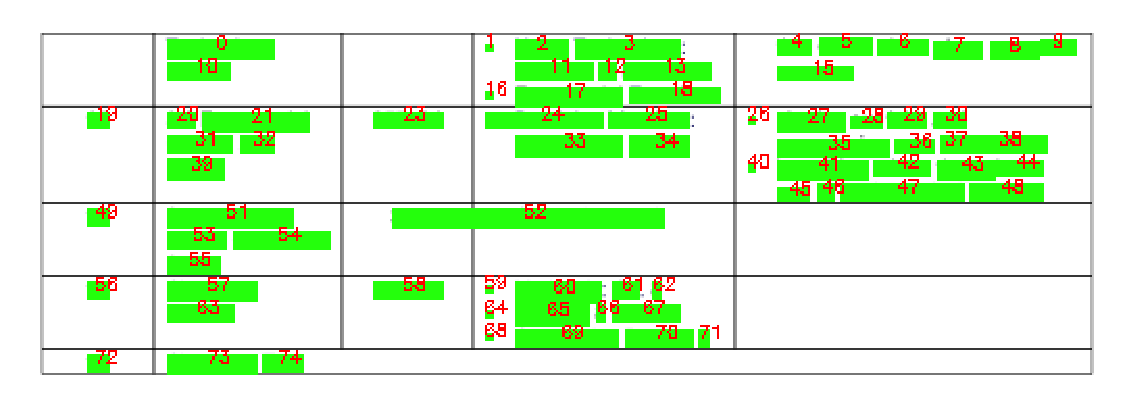
\includegraphics[width=\textwidth]{images/chapter4/tesseract_tables.pdf}
        \caption{Reading order obtained through Tesseract}
      \end{subfigure}
    \caption{Ground-truth reading order (a) compared to the reading order generated by Tesseract (b) for a sample table. Non-highlighted text indicates that it does not appear in the serialized sequence.}
    \label{fig:reading-orders-table}
\end{figure}

\begin{figure}[!htbp]
  \centering
  \small
      \begin{subfigure}[b]{0.5\textwidth}
        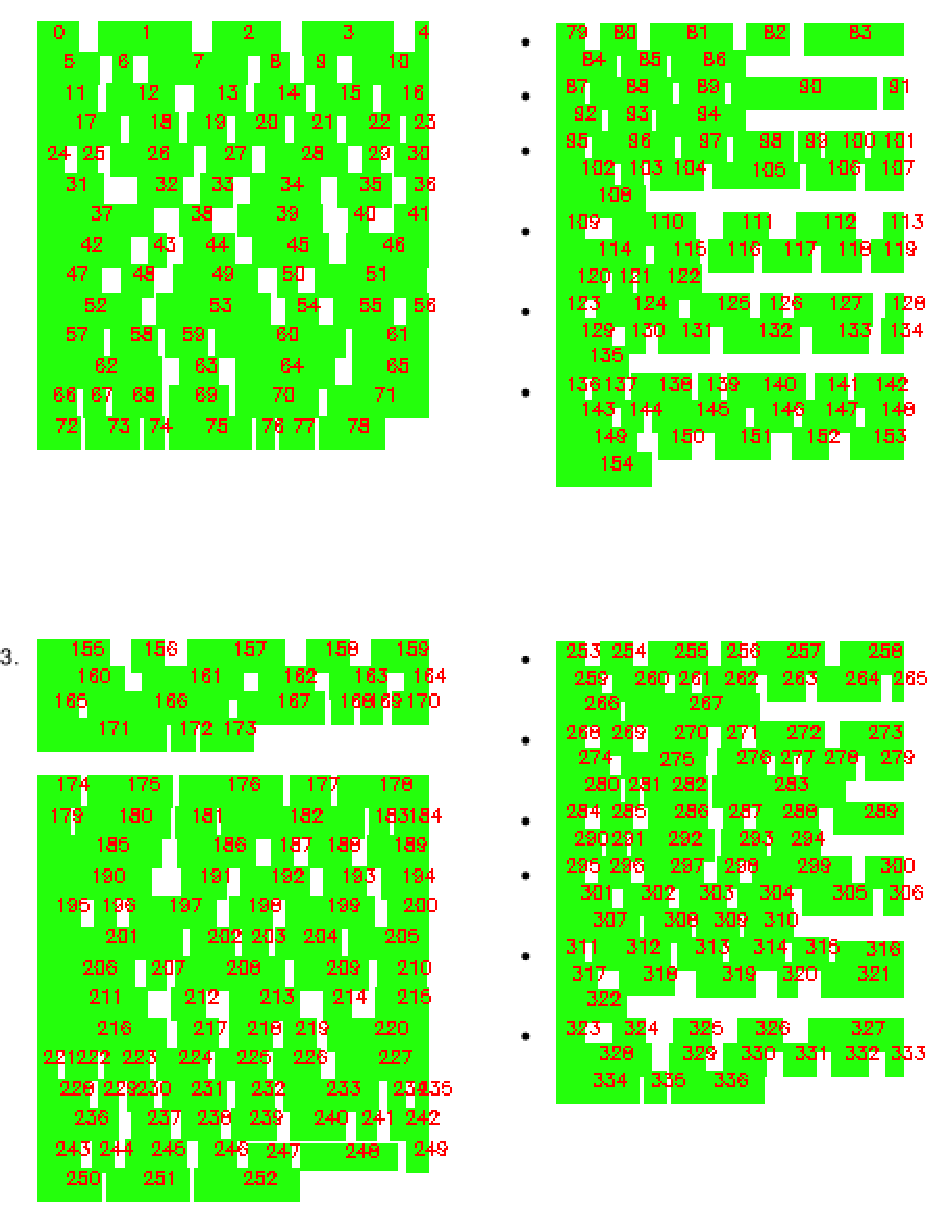
\includegraphics[width=\textwidth]{images/chapter4/gold_multicolumn.pdf}
        \caption{Ground-truth}
      \end{subfigure}
      \begin{subfigure}[b]{0.5\textwidth}
        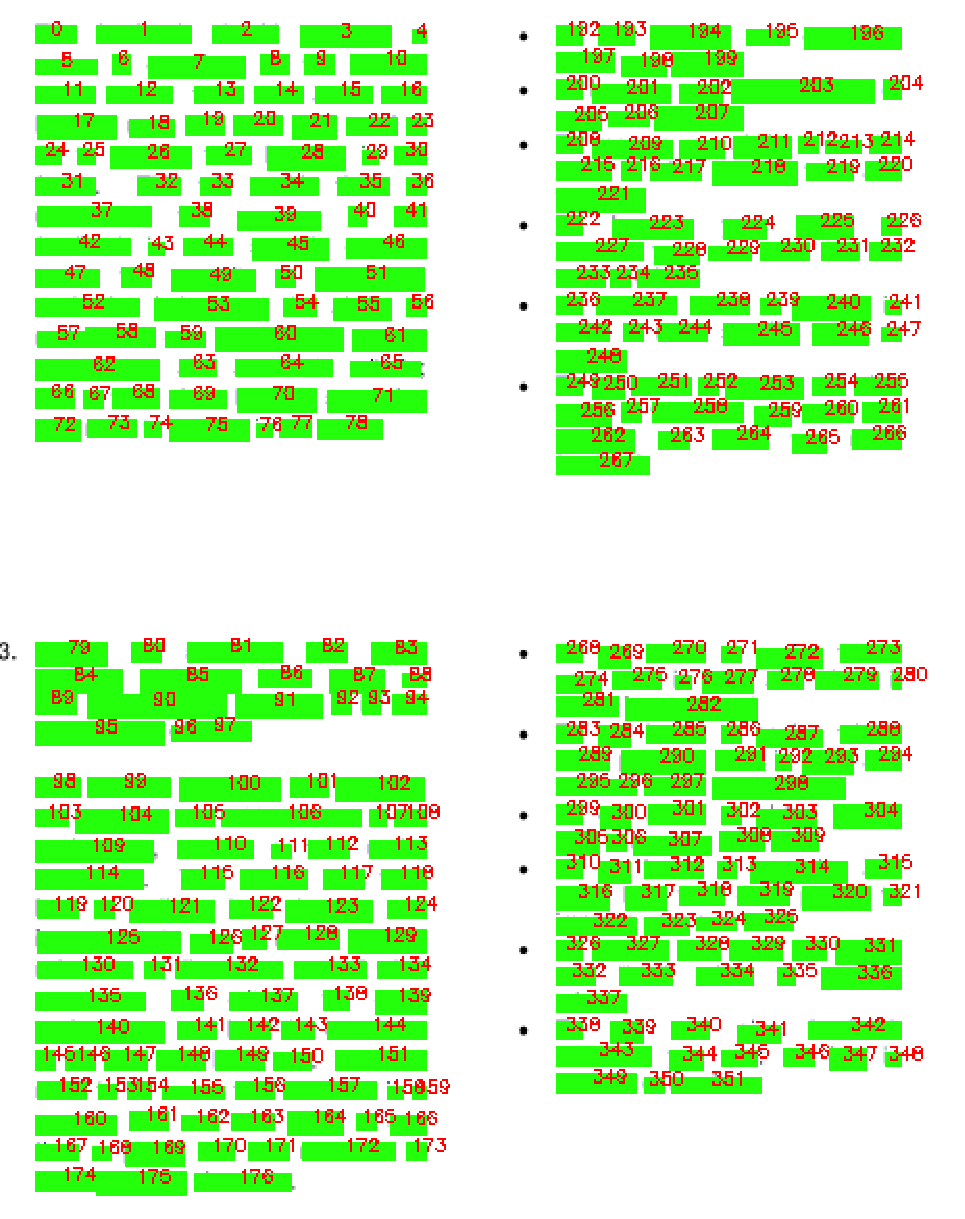
\includegraphics[width=\textwidth]{images/chapter4/tesseract_multicolumn.pdf}
        \caption{Tesseract}
      \end{subfigure}
    \caption{Ground-truth reading order (a) compared to the reading order generated by Tesseract (b) for a document with a two-column layout. The document was cropped for better visibility. Non-highlighted text indicates that it does not appear in the serialized sequence.}
    \label{fig:reading-orders-multicolumn}
\end{figure}


\subsection{Layout2Pos Module}

Building on the insights gained from the previous experiment, accurately retrieving the correct reading order poses a significant challenge for \ac{OCR} systems. We argue that it is possible to retrieve the correct reading order by leveraging the document layout. To address this, we propose a novel approach, \textit{Layout2Pos}, a transformer-based module that discards the reading order generated by \ac{OCR} and, instead, learns 1D position embeddings exclusively from the spatial positions of tokens. Layout2Pos is a stack of Transformer layers designed to take a sequence of token layout embeddings and generate a corresponding sequence of 1D position embeddings. In the following, we elaborate on the process of encoding spatial information into layout embeddings, followed by an in-depth description of our Layout2Pos module.

\subsubsection{Encoding Layout Information}

The spatial position of a token is represented by its bounding box in the document page image, denoted as $(x_0, y_0, x_1, y_1)$, where $(x_0, y_0)$ and $(x_1, y_1)$ correspond to the coordinates of the top-left and bottom-right corners, respectively. We discretize and normalize these coordinates to integers within the range of $[0, ..., 1000]$. Four embedding tables are employed to encode spatial positions: two for the coordinate axes ($x$ and $y$), and the other two for the bounding box size (width and height). In line with LayoutLMv2 \citep{xu2020layoutlmv2}, the final layout embedding $\bell \in \mathbb{R}^{d_{\ell}}$ of a token positioned at $(x_0, y_0, x_1, y_1)$ is defined as follows:

\begin{equation}
\begin{split}
    \bell & = \text{LayoutEmb}_x(x_0) \mathbin\Vert \text{LayoutEmb}_y(y_0) \\
    & \mathbin\Vert \text{LayoutEmb}_x(x_1) \mathbin\Vert \text{LayoutEmb}_y(y_1) \\
    & \mathbin\Vert \text{LayoutEmb}_w(x_1 - x_0) \mathbin\Vert \text{LayoutEmb}_h(y_1 - y_0), 
\end{split}
\label{eq:layout-embeddings}
\end{equation}

\noindent where $\mathbin\Vert$ denotes concatenation.

Following LayoutLMv2, we also encode spatial relative positions as bias terms added to the attention scores to explicitly capture the spatial relationship between tokens. For each pair of bounding boxes $((x_0, y_0, x_1, y_1), (x^{\prime}_0, y^{\prime}_0, x^{\prime}_1, y^{\prime}_1))$, we compute the horizontal distance $x^{\prime}_0 - x_0$ between the left edge of each box and the vertical distance $y^{\prime}_1 - y_1$ between the bottom edge of each box. To provide additional insights into the spatial relationships of tokens, we also compute the horizontal distance $x^{\prime}_1 - x_0$ between the right edge of one box and the left edge of the other (indicating information about the combined length). Furthermore, we calculate the horizontal distance $x^{\prime}_1 - x_1$ between the right edge of each box, providing information about the length of the second token in the pair. In addition, we consider \textit{line} and \textit{column} relative positions. Understanding the relative positions within lines helps the sequential structure of the document, aiding in distinguishing between different parts of the document. On the other hand, the relative positions within columns is valuable for documents with multicolumn layouts, offering insights into the spatial arrangement of text across columns. Overall, line and column information enhance the model's ability to capture the structural organization of textual content within documents. Hence, for each bounding box, we identify other bounding boxes that share the same line/column. This is determined by whether the horizontal/vertical line passing through the center of the box intersects with the other bounding boxes. If there is an intersection, the boxes are considered to be on the same line/column. For each token, we determine its positions within its corresponding line and column. Then, we compute the relative sequential distance $\delta^{line}_{ij}$ and $\delta^{column}_{ij}$ between elements within each line and column. If they do not belong to the same line or column, the distance is set to 1000. 

Formally, let $\bm{q}^{\ell}_i$ and $\bm{k}^{\ell}_i$ denote the query and key projections obtained from the layout embedding $\bell_i$ of token $i$. In Layout2Pos, attention is re-defined as:

\begin{equation}
  \begin{split}
  \alpha_{ij} &= \dfrac{1}{\sqrt{d}} \left(\bm{q}^{\ell}_i \cdot \bm{k}^{\ell}_j\right) \\
              & + b^{(2D_x)}_{x^{(j)}_{0} - x^{(i)}_{0}} + b^{(2D_y)}_{y^{(j)}_{1} - y^{(i)}_{1}} + b^{(2D_x)}_{x^{(j)}_{1} - x^{(i)}_{0}} + b^{(2D_x)}_{x^{(j)}_{1} - x^{(i)}_{1}} \\
              & + b^{(l)}_{\delta^{l}_{ij}}  + b^{(c)}_{\delta^{c}_{ij}},
  \end{split}
  \label{eq:layout2pos-attention}
\end{equation}

\noindent where $\bm{b}^{(2D_x)}$, $\bm{b}^{(2D_y)}$, $\bm{b}^{(l)}$, and $\bm{b}^{(c)}$correspond to the horizontal, vertical, line, and column relative position biases, respectively. The biases are different among attention heads but shared across all layers. The relative sequential distances between elements within lines and columns, $\bm{\delta}^{(line)}$ and $\bm{\delta}^{(column)}$, are defined as follows:

\begin{equation}
  \begin{split}
    \delta^{l}_{ij} &= 
        \begin{cases}
          posInLine(j) - posInLine(i), & \text{if } line(j) = line(i)\\
            1000,              & \text{otherwise}.
        \end{cases} \\
    \delta^{c}_{ij} &= 
      \begin{cases}
        posInColumn(j) - posInColumn(i), & \text{if } column(j) = column(i)\\
          1000,              & \text{otherwise}.
      \end{cases}
  \end{split}
\end{equation}

\subsubsection{Learning 1D Position Embeddings from Layout Information}

\begin{figure}[h]
  \centering
  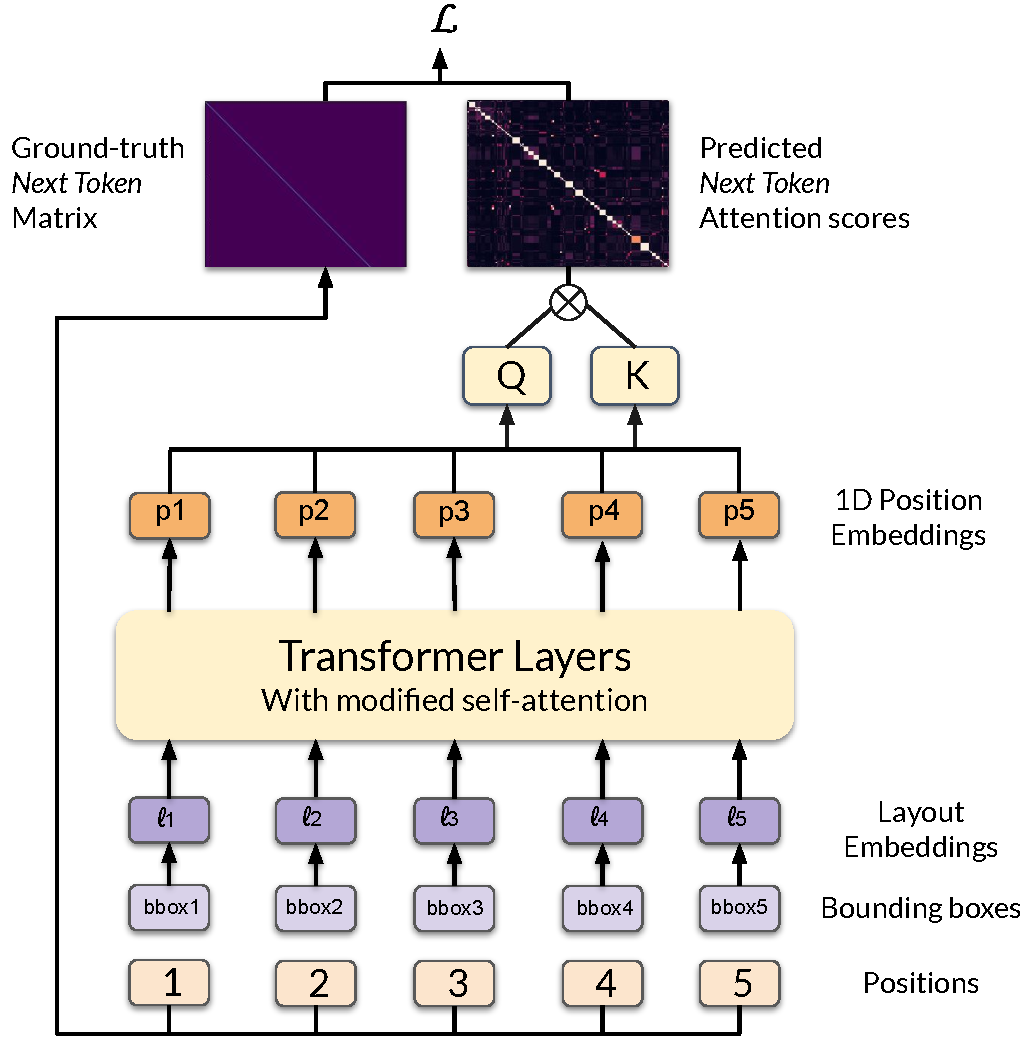
\includegraphics[width=0.75\textwidth]{images/chapter4/Layout2Pos.pdf}
  \caption{Layout2Pos Architecture. The input consists of a sequence of token bounding box coordinates, transformed into corresponding embedding sequences. Self-attention in the stack of Transformer layers is modified as defined by Equation~\ref{eq:layout2pos-attention}. $\bm{Q}$ and $\bm{K}$ are the queries and keys obtained by projecting the 1D position embeddings. The attention scores obtained through dot-product are compared against the ground-truth matrix to compute the Next Token Prediction score.}
\end{figure}

Given a sequence of layout embeddings as defined by Equation~\ref{eq:layout-embeddings}, Layout2Pos employs a stack of $M$ Transformer layers to contextualize the sequence. The outputs of the last layer serve as 1D position embeddings:

\begin{equation}
  \bm{p}_i = \bm{h}^M(\bell_i).
\end{equation}

\noindent Then, these 1D position embeddings are used to compute the attention matrix $\bm{A}$, \textit{i.e.}, alignment scores between every token:

\begin{equation}
  A_{ij} = \left(\bm{p}_i \bm{W}^q\right)\left(\bm{p}_j \bm{W}^k\right).
\end{equation}

\noindent We assume that the attention matrix $\bm{A}$ carries information about the reading order, \textit{i.e.}, $A_{ij}$ represents the probability that the $j$-th token follows the $i$-th token. Let $N$ denote the ground-truth binary matrix where $N_{ij}$ equals $1$ if token $j$ is the \textit{next} token after token $i$ in the sequence, and $0$ otherwise. We define the \textit{Next Token Prediction} strategy, which consists in using the attention matrix $\bm{A}$ to predict the next token of each token in the sequence. The corresponding loss is defined as follows:

\begin{equation}
  \mathcal{L}_{NTP} = - \sum_{i=1}^n \sum_{j=1}^n N_{ij} \log\left(\textrm{softmax}(A_{ij})\right).
\end{equation}

\noindent As such, Layout2Pos is trained to capture the relationship between spatial arrangement of tokens and reading order. This is done ensuring that the attention matrix $\bm{A}$ derived from the computed 1D position embeddings carries information about the next token for each token in the sequence. It is noteworthy that that a global reading order is unnecessary; there is no requirement to establish an order between two words that belong to segments that have no relation to each other.

Given that each token is treated as a bounding box defined by its size and position, a significantly smaller representation space can be chosen for layout features compared to text. As Layout2Pos does not need to understand semantic content, it may require a smaller latent space dimension than conventional multimodal pre-trained models. 

The 1D position embeddings generated by Layout2Pos can be incorporated into the inputs of a Transformer-based language model, serving as an alternative to traditional 1D position encodings derived from an OCR-induced reading order.


\section{Experiments and Results}

\subsection{Data}

\subsubsection{Pre-training Data}

Following a common practice in the field of Document Understanding, we collect data from the IIT-CDIP collection \citep{lewis2006building} to build our pre-training dataset. IIT-CDIP consists of around 11 million document page images of various types and layouts, including news articles, scientific reports, and handwritten materials. The collection contains scanned images of documents, introducing challenges related to image quality, resolution, and potential artifacts. As such, we leverage the IIT-CDIP collection to evaluate the generalization and performance of models under realistic conditions. We select 7 million document images from the collection to build our pre-training dataset. To extract text and bounding boxes from the documents, we use DocTR \citep{doctr2021}, a package of robust two-stage \ac{OCR} systems.

% IIT-CDIP not used for next token prediction

Because Layout2Pos needs to be trained with documents where the reading order aligns with human reading patterns, we also use the ReadingBank dataset \citep{wang2021layoutreader} to pre-train our models. 

\subsubsection{Data for Visual Information Extraction}

\subsection{Experimental Settings}

\subsection{Next Token Prediction}

\subsection{Visual Information Extraction}

\section{Conclusion}